\section{Experiments}

\subsection{Implementation Details}
We implement AnyFlow on top of Wan2.1~\cite{wan2025wan} in the Diffusers framework~\cite{von-platen-etal-2022-diffusers}. We train the model on a synthetic dataset of 256K prompt--video pairs generated from Wan2.1-T2V-14B, where each sample contains up to 81 frames at a resolution of $480 \times 832$. Training is performed in two stages. In Stage 1, we optimize the forward flow map objective using AdamW~\cite{loshchilov2017decoupled} with a learning rate of $5 \times 10^{-5}$ and a global batch size of 32 for the 1.3B model and 16 for the 14B model, for 6,000 and 4,000 iterations, respectively. In Stage 2, we perform on-policy distillation by jointly optimizing the forward flow map and on-policy objectives with AdamW at a learning rate of $2 \times 10^{-6}$ for 800 iterations. In both stages, we use parameter-efficient fine-tuning with LoRA~\cite{hu2022lora} of rank 256.

\subsection{Evaluation Setting}
For text-to-video (T2V) evaluation, we adopt VBench~\cite{huang2023vbench}, which evaluates generation quality across 16 fine-grained dimensions grouped into two high-level categories: Quality score and Semantic score. For image-to-video (I2V) evaluation, we use VBench-I2V~\cite{huang2025vbench++} and report both the Quality score and the I2V score.

To ensure a fair comparison, we re-evaluate key counterparts under a unified protocol using the official VBench augmented prompts. These counterparts include the Wan2.1 base model~\cite{wan2025wan}, Self-Forcing~\cite{huang2025selfforcing}, and rCM~\cite{zheng2025large}, as well as community-trained 14B causal models including FastVideo~\cite{causalwan2025}, Krea-Realtime-14B~\cite{krea_realtime_14b}, and LightX2V~\cite{lightx2v}. Results for all other methods are taken directly from their original papers.
\subsection{Main Results}
\myPara{Quantitative Comparison.}
As shown in \cref{tab:t2v_comparison}, AnyFlow achieves strong few-step performance and continues to improve as the sampling budget increases. On the 14B bidirectional backbone, AnyFlow-Wan2.1-T2V-14B obtains 84.04 at 4 NFEs, outperforming rCM-Wan2.1-T2V-14B (83.73 at 4 NFEs). On the 14B causal backbone, AnyFlow-FAR-Wan2.1-14B reaches 84.05 at 4 NFEs and further improves to 84.41 at 32 NFEs, outperforming strong community counterparts.

For image-to-video results in \cref{tab:i2v_comparison}, AnyFlow-FAR-Wan2.1-14B achieves a VBench-I2V score of 87.87 using only 4 NFEs. This result is comparable to Wan2.1-I2V-14B with 50$\times$2 NFEs (87.71) and surpasses FastVideo-CausalWan2.2-A14B-Preview (86.82), showing that AnyFlow improves both visual quality and I2V faithfulness while retaining strong sampling efficiency.

\myPara{Qualitative Comparison.}
As shown in \cref{fig:14b_compare}, we provide qualitative comparisons at the 14B scale for both T2V and I2V generation. In causal T2V examples, FastVideo-Wan2.2-A14B-Preview exhibits blurry details, LightX2V-Wan2.1-14B-CausVid shows flickering artifacts, and Krea-Realtime-14B produces unrealistic motion in some clips. By comparison, AnyFlow-FAR-Wan2.1-14B delivers the best visual quality and motion with 4 NFEs. In bidirectional T2V examples, AnyFlow-Wan2.1-T2V-14B shows slightly better motion than rCM-Wan2.1-T2V-14B.

For I2V generation, AnyFlow reuses the causal generator through our non-uniform chunk partition and maintains good first-frame faithfulness with smooth motion transitions. Compared with Wan2.1-I2V-14B, AnyFlow-FAR-Wan2.1-14B shows comparable temporal stability and motion quality, while FastVideo-Wan2.2-A14B-Preview exhibits visible flickering and inconsistencies with the input image. Overall, these qualitative results are consistent with the quantitative trends and further support the effectiveness of AnyFlow in few-step sampling.

\begin{figure}[!tb]
    \centering
    \begin{subfigure}{0.45\textwidth}
        \centering
        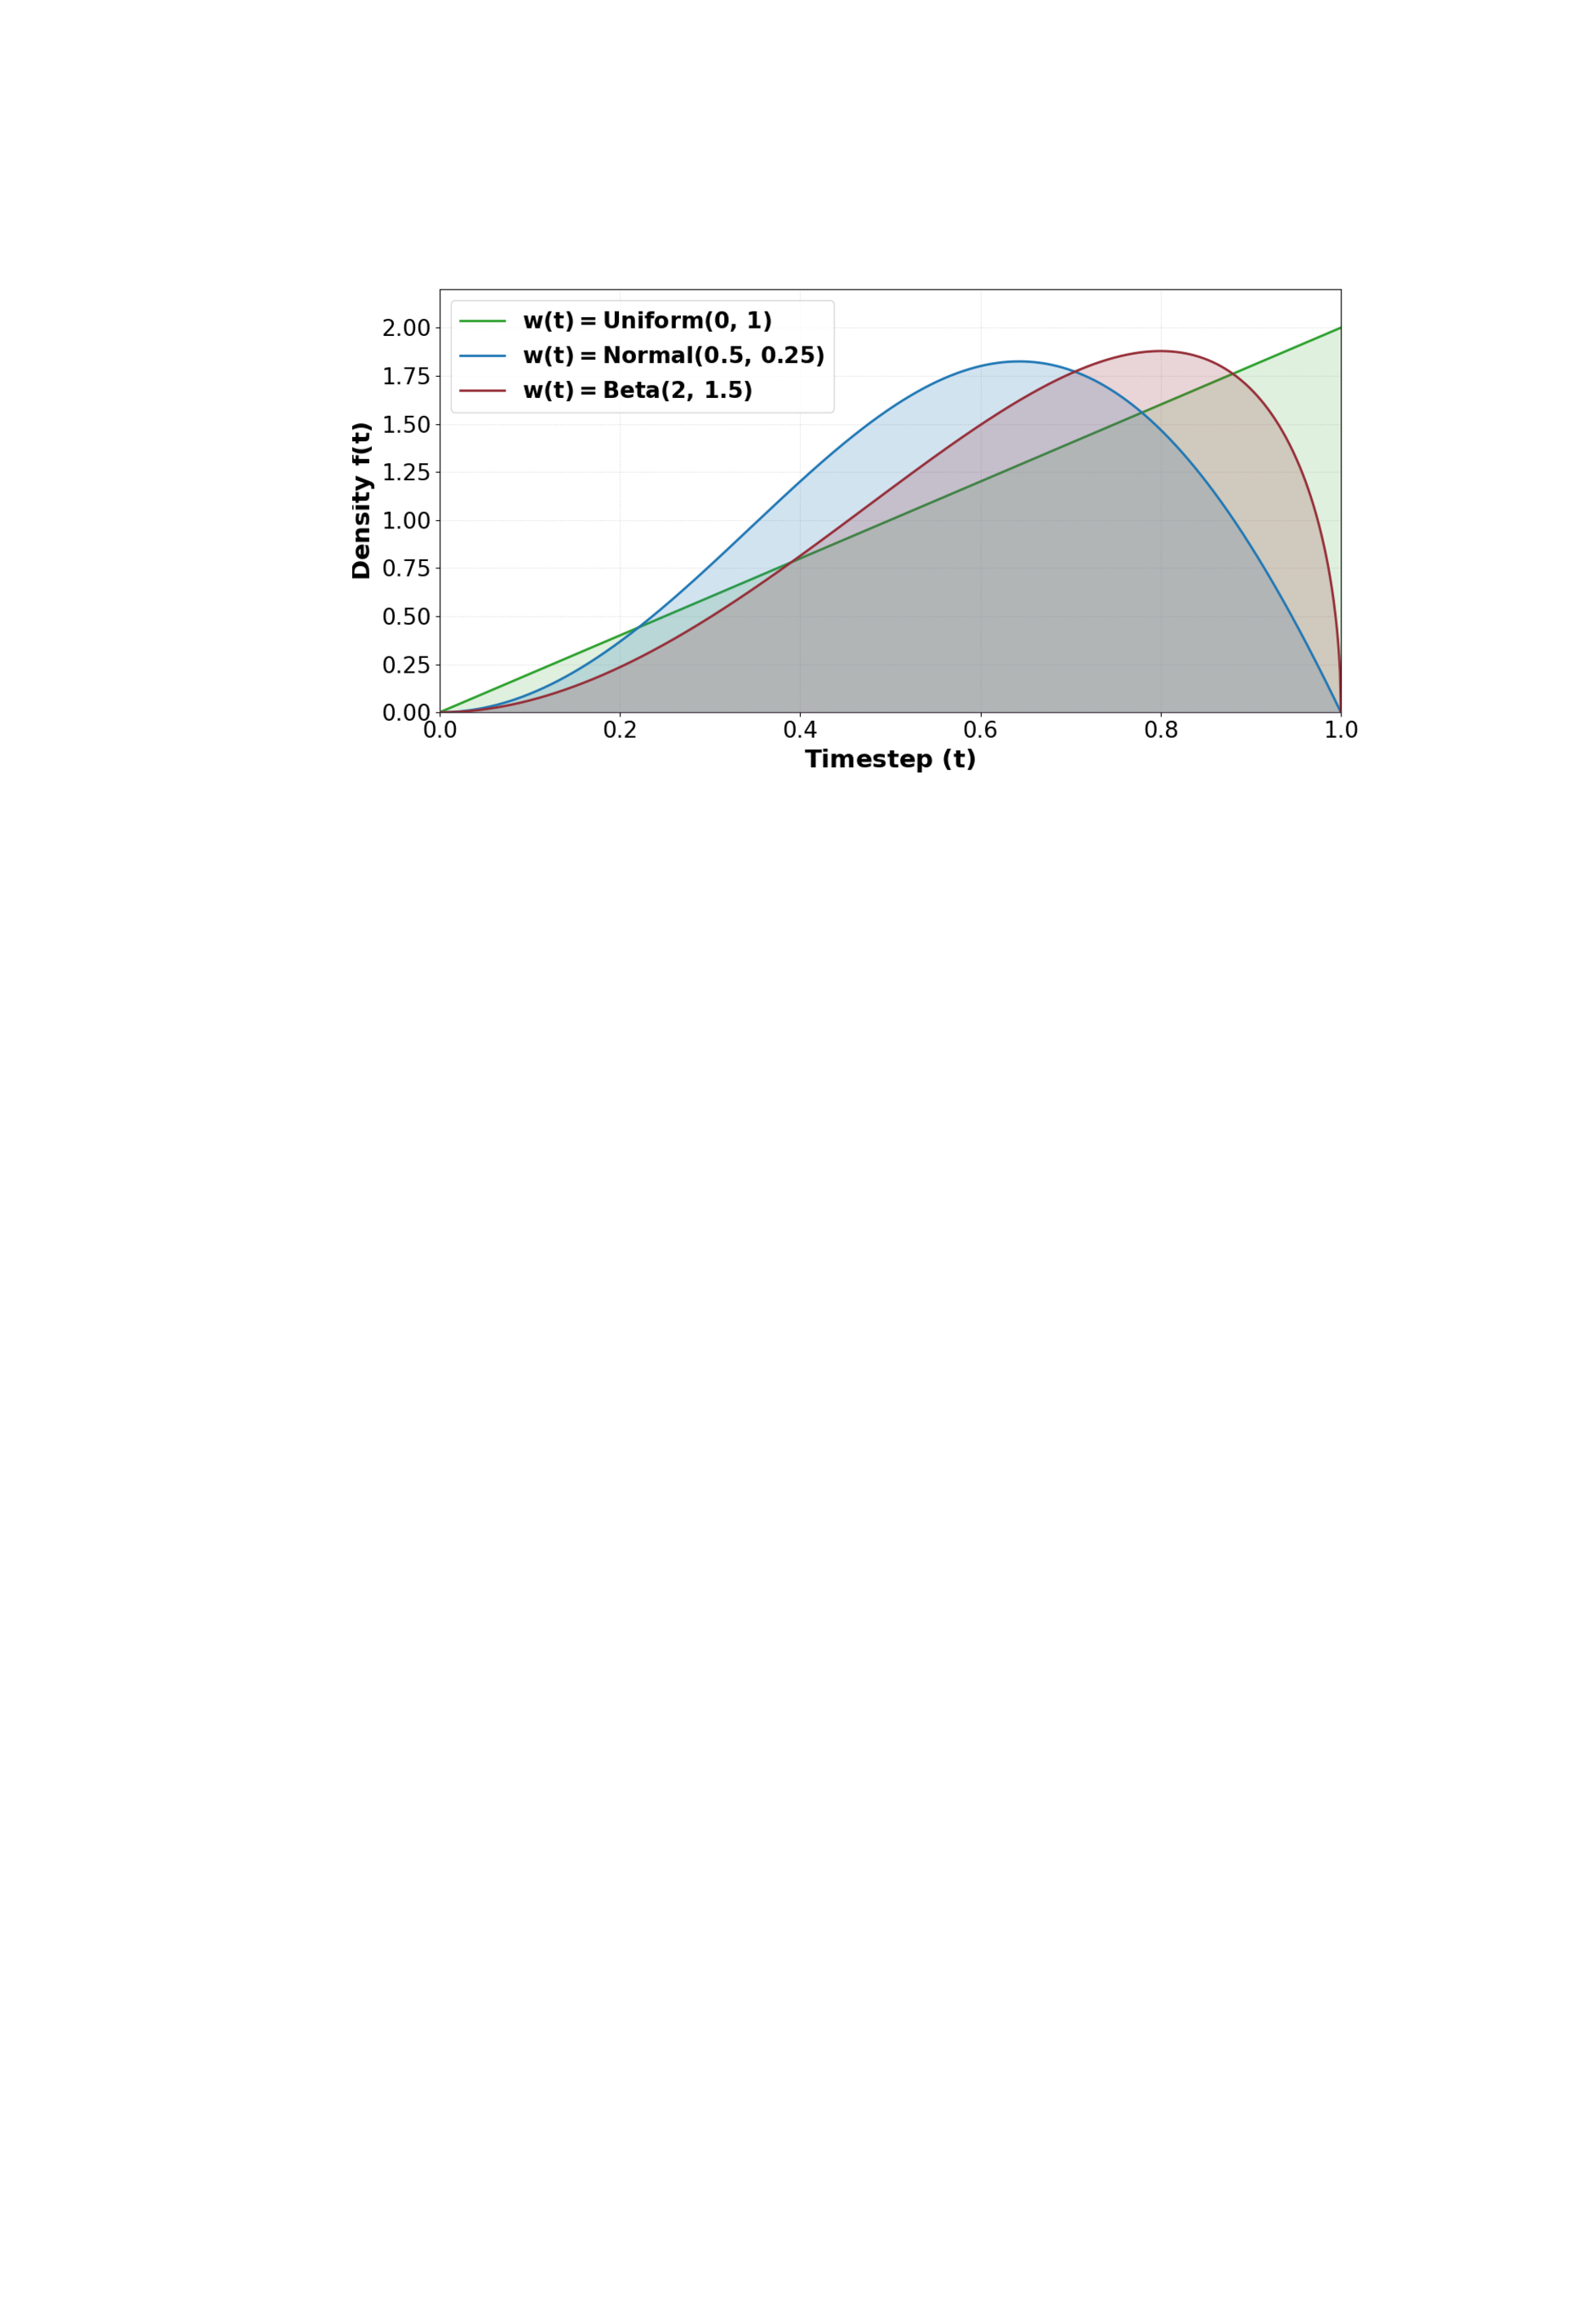
\includegraphics[width=\textwidth]{figures/src/time_sampler.pdf}
        \caption{Timestep density $f(t)=p(t)\cdot w(t)$, where $p(t)=2t$.}
        \label{fig:vis_distribution}
    \end{subfigure}
    \hfill
    \begin{subtable}{0.53\textwidth}
        \centering
\renewcommand{\arraystretch}{1.55}
        \resizebox{\linewidth}{!}{\begin{tabular}{l|cc|cc}
    \toprule
    \multirow{2}{*}{$\mathbf{w(t)}$} & \multicolumn{2}{c|}{\textbf{Bidirectional}} & \multicolumn{2}{c}{\textbf{Causal}} \\
    \cmidrule(lr){2-3} \cmidrule(lr){4-5}
    & \textbf{4 NFEs} & \textbf{32 NFEs} & \textbf{4 NFEs} & \textbf{32 NFEs} \\
    \midrule
    $\text{Uniform}(0, 1)$    & 83.46 & 83.75 & \textbf{83.58} & 83.91 \\
    $\text{Normal}(0.5, 0.25)$  & 83.40 & 83.79 & 83.54 & 83.93 \\
    \rowcolor{mitblue}$\text{Beta}(2, 1.5)$   & \textbf{83.48} & \textbf{83.96} & 83.54 & \textbf{83.96} \\
    \bottomrule
\end{tabular}}
        \caption{Quantitative ablation (Vbench overall score) of the loss weight function $w(t)$.}
        \label{tab:ablation_time_sampler}
    \end{subtable}
    \caption{\textbf{Ablation Study of Loss Weight Function $w(t)$}. Among the different weighting strategies, $w(t) = \text{Beta}(2, 1.5)$ demonstrates the best performance across both architectures.}
\label{fig:ablation_time_sampler}
\end{figure}
\begin{figure}[!tb]
    \centering
    \begin{subfigure}{\textwidth}
        \centering
        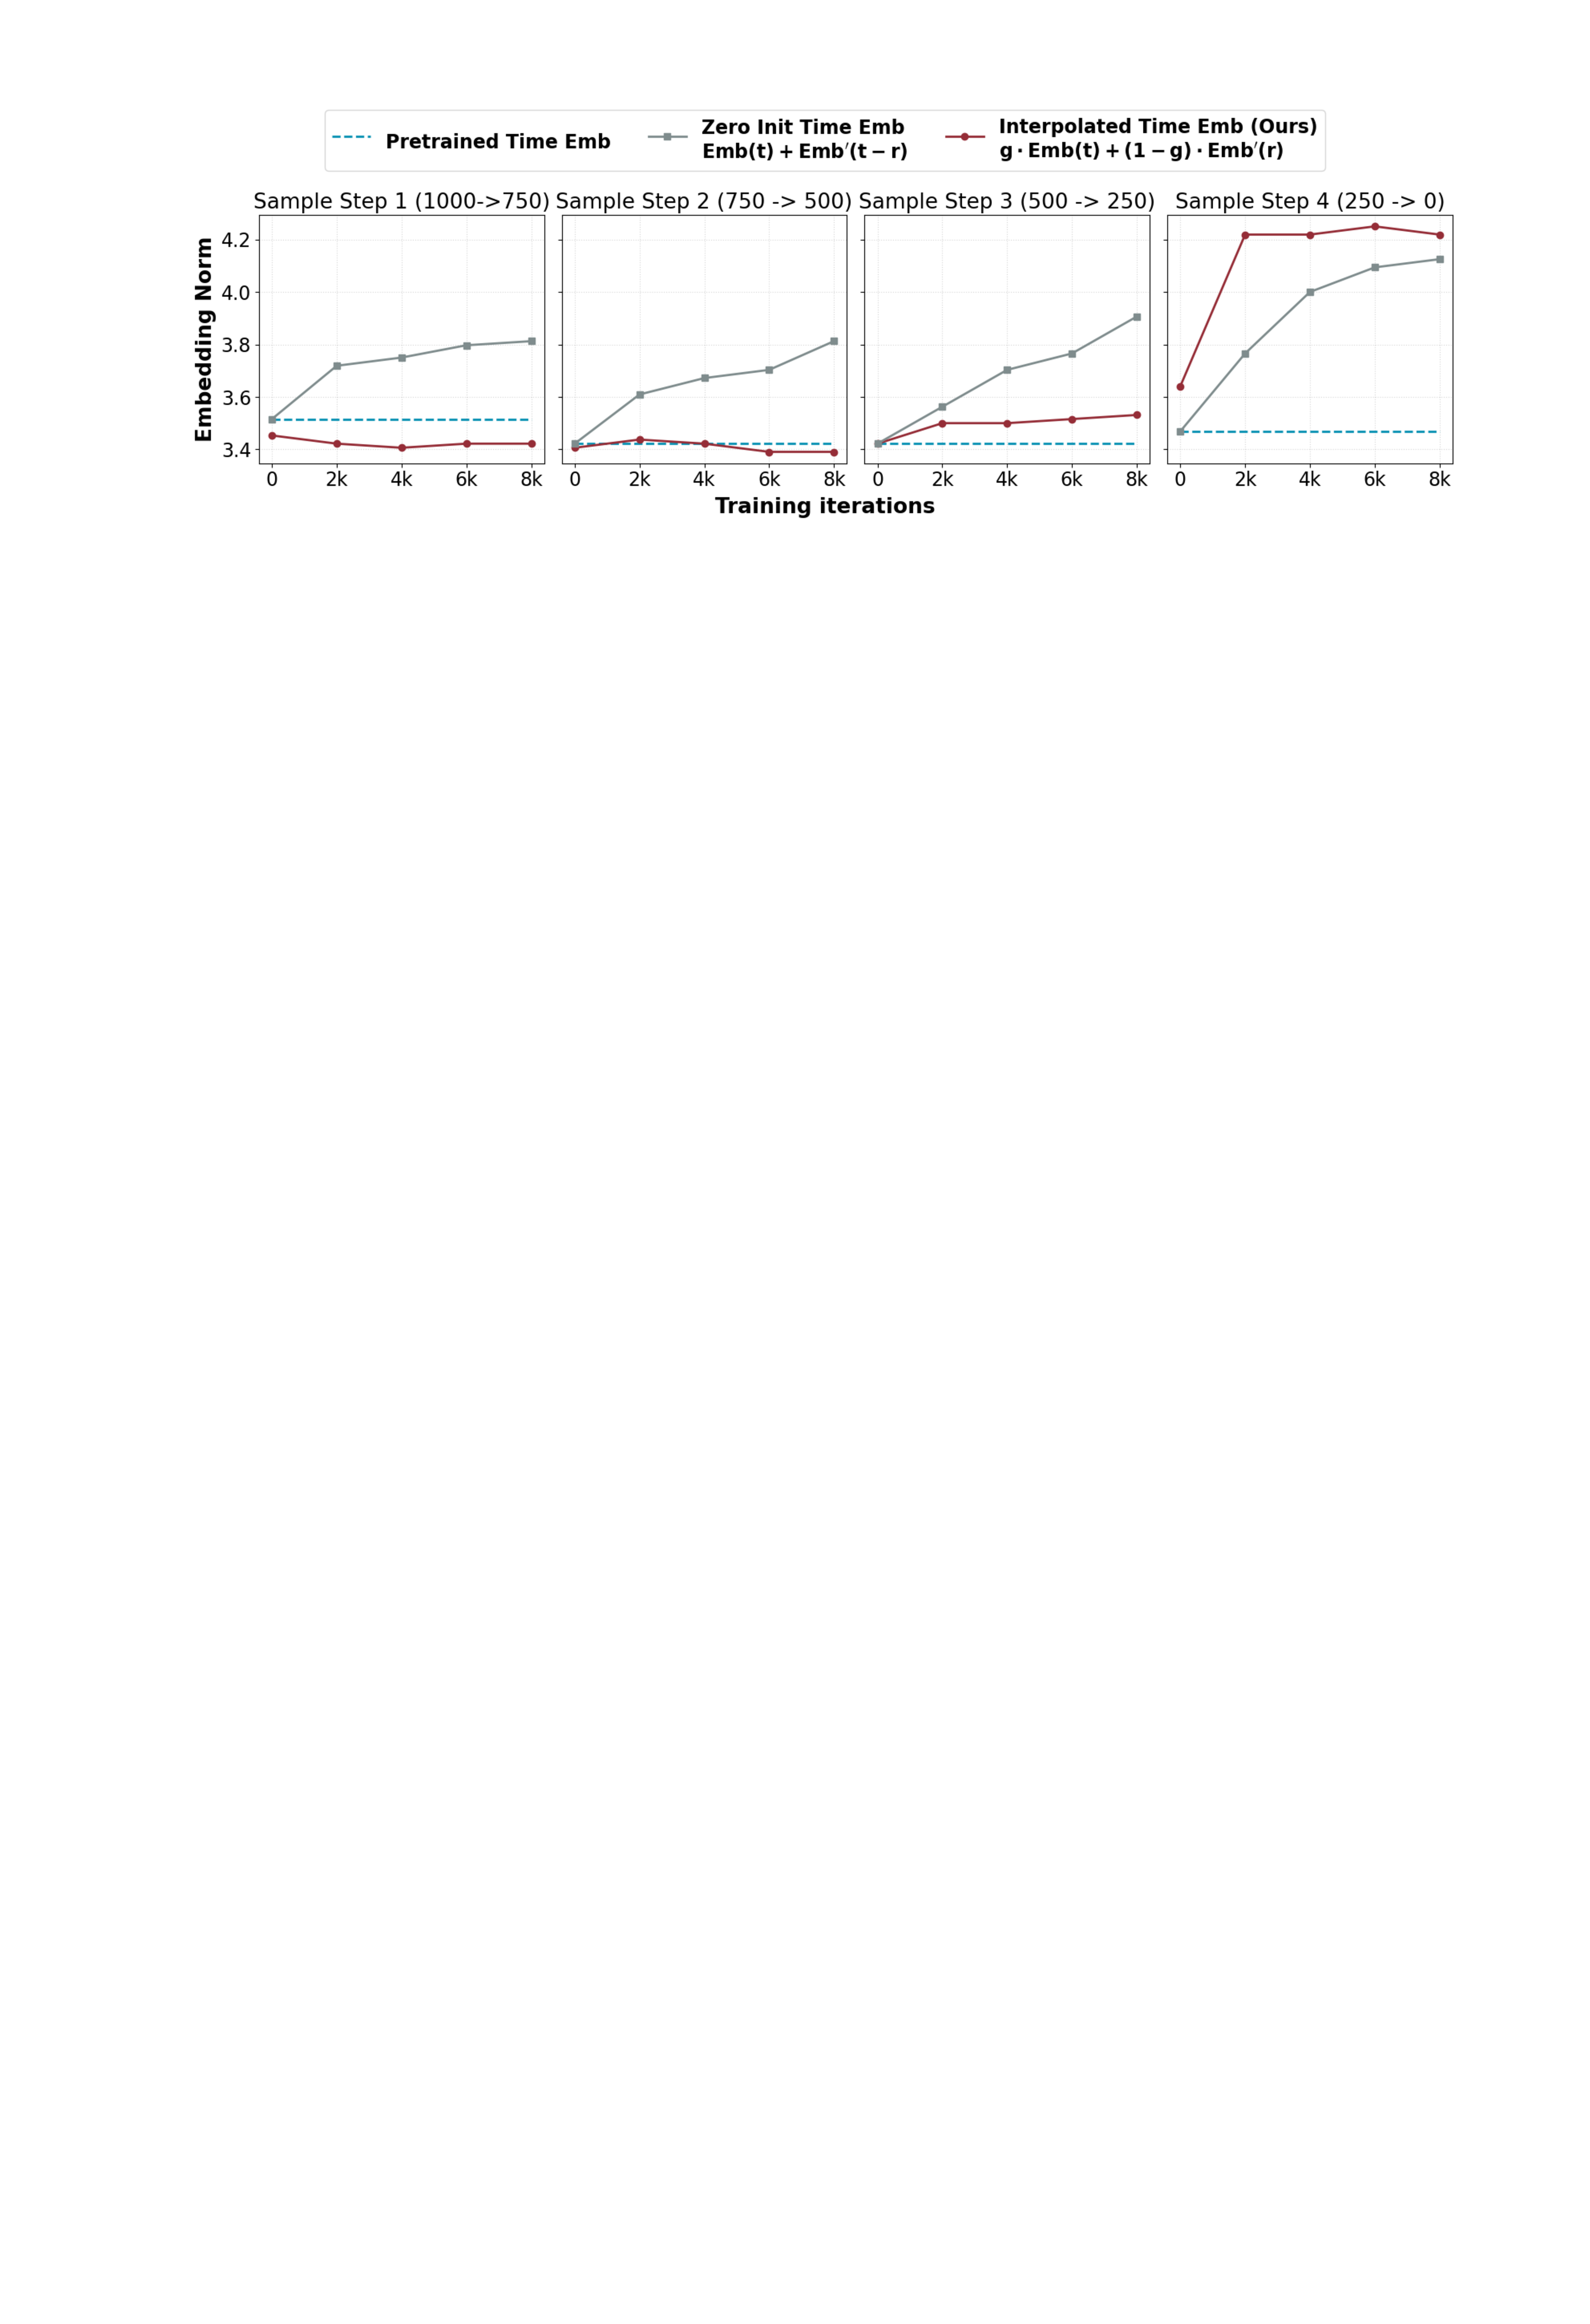
\includegraphics[width=\textwidth]{figures/src/interpolated_embedding.pdf}
        \caption{Comparison of embedding norms at different sample steps during training.}
        \label{fig:interpolated_time_norm}
    \end{subfigure}
    
    \begin{subfigure}{\textwidth}
        \centering
        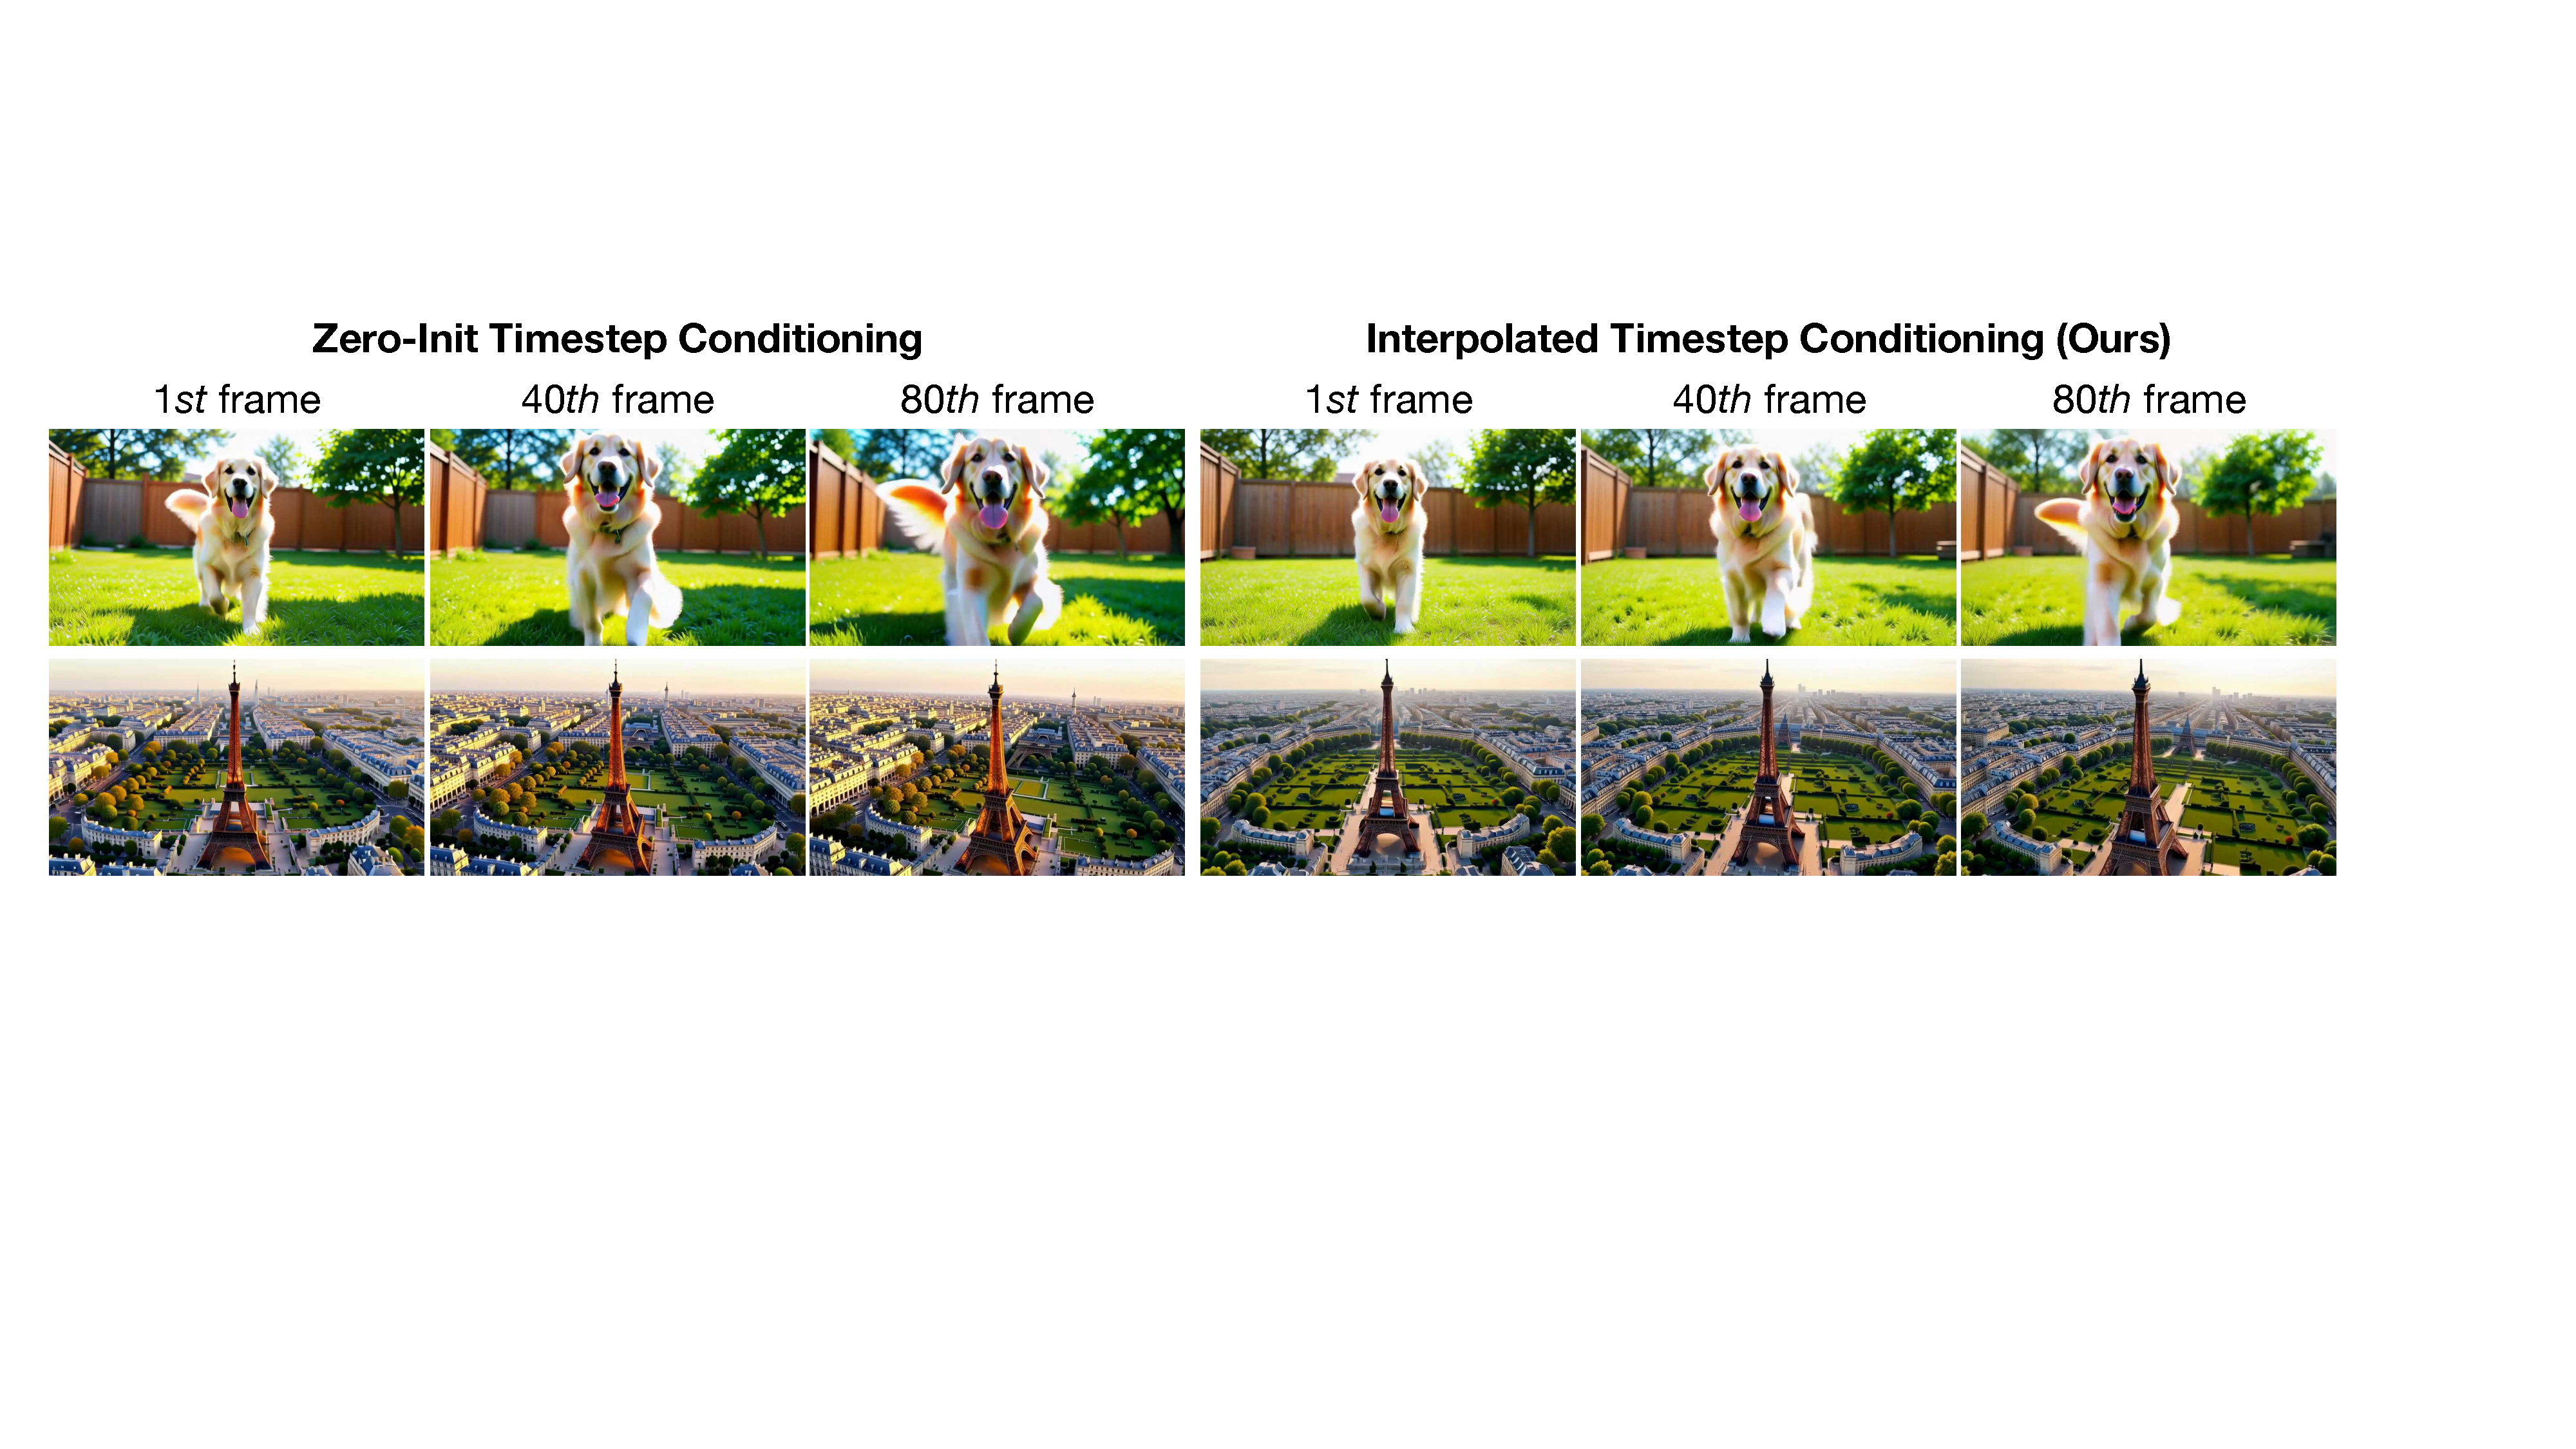
\includegraphics[width=\textwidth]{figures/src/interpolated_visualization.pdf}
        \caption{Visual comparison of zero-init timestep conditioning and interpolated timestep conditioning.}
        \label{fig:interpolated_time_vis}
    \end{subfigure}
    \caption{\textbf{Ablation Study of Timestep Conditioning}. Compared with zero-init timestep conditioning, the proposed interpolated method achieves embedding norms more consistent with pretrained embeddings, preventing over-saturated visual results.}
    \label{fig:ablation_interpolated_time}
\end{figure}

\subsection{Ablation Study}
\myPara{Time Sampler.}
We investigate different choices of the time sampler, with their induced densities over $t$ visualized in \cref{fig:vis_distribution}. The uniform weighting yields the worst test-time scalability, as reflected by its 32-step performance in \cref{tab:ablation_time_sampler}, likely because it mismatches the logit-normal time weighting used in pretraining. Among the other variants, assigning more probability mass to high-noise regions leads to better overall performance. Therefore, we fix $w(t)=\text{Beta}(2, 1.5)$ in all experiments.

\myPara{Interpolated Timestep Conditioning.} Incorporating an additional timestep embedding during post-training is non-trivial. A baseline design is to add a new embedding projection whose final layer is zero-initialized, as in TMD~\cite{nie2026transition}. However, under zero initialization, the model needs to amplify the influence of the $r$ embedding, which causes its norm to keep increasing during training and eventually leads to over-saturated results, as shown in \cref{fig:ablation_interpolated_time}. In contrast, our interpolated timestep conditioning preserves the boundary case $t=r$ for stability while avoiding an overly cold start when $t\neq r$. As a result, the embedding norm remains stable after roughly 2K training steps and stays much closer to that of the pretrained model, effectively suppressing the over-saturation effect.

\begin{figure*}[!tb]
  \centering
  \animategraphics[width=\linewidth]{8}{figures/videosrc/ablation_odeinit/}{00000}{00020}
  \vspace{-.3in}\caption{\textbf{Qualitative Ablation Study of ODE-Init and AnyFlow on Causal Video Generation.} Readers can \textcolor{magenta}{click and play} the video clips in this figure using Adobe Acrobat.}
  \label{fig:ablation_odeinit}
\end{figure*}

\myPara{Comparison to ODE-Init.}
We compare AnyFlow with Consistency ODE-Init for causal video generation in \cref{fig:ablation_odeinit}. For a fair comparison, we fine-tune the teacher on the same synthetic dataset, since we do not have access to the original training data of the Wan base model. After flow map training, AnyFlow produces clearer results than Consistency ODE-Init at both 4 and 32 NFEs, indicating that it better preserves the knowledge inherited from the flow-matching-pretrained base model. After on-policy distillation, AnyFlow further reduces test-time errors in few-step sampling and improves the overall sampling trajectory. We also observe that our method preserves the style and content of the pretrained model more faithfully.

\begin{table}[!tb]
    \centering
    \resizebox{0.85\linewidth}{!}{
    \begin{tabular}{l|ll}
        \toprule
        \multirow{2}{*}{\textbf{Method}} & \multicolumn{2}{c}{\textbf{Training Cost (s/iter on H100)}} \\
        \cmidrule{2-3}
         & \textbf{Causal} & \textbf{Bidirectional} \\
        \midrule
        \midrule
        \multicolumn{3}{c}{\textbf{Forward Training}} \\
        \midrule\midrule
        Standard Flow-Matching & 5.8 & 9.7 \\
        + Guidance-Fused Training & 7.8 & 12.3 \\
        \rowcolor{mitblue}+ Guidance-Fused Training + Differential Derivation Equation & 10.4 & 16.8 \\
        \midrule
        \midrule
        \multicolumn{3}{c}{\textbf{On-Policy Distillation}} \\
        \midrule\midrule
        Consistency Backward Simulation (4 Steps) & 45.9 & 41.8 \\
        \rowcolor{mitblue}Flow Map Backward Simulation (4 Steps) & 53.1 (\textcolor{red}{+15.7\%}) & 51.2 (\textcolor{red}{+22.5\%}) \\\midrule
        Consistency Backward Simulation (16 Steps) & 93.8 & 96.6 \\
        \rowcolor{mitblue}Flow Map Backward Simulation (16 Steps) & 53.1 (\textcolor{green!50!black}{-43.4\%}) & 51.2 (\textcolor{green!50!black}{-47.0\%}) \\
        \bottomrule
    \end{tabular}}
      \caption{\textbf{Training Cost Breakdown of AnyFlow.} Costs are measured on Wan2.1-1.3B-T2V with batch size 16 on a node with 8$\times$NVIDIA H100 GPUs. During on-policy distillation, we evaluate the upper-bound cost (comprising one generator and one discriminator update) for the  simulation trajectories.}

    \label{tab:train_cost}
\end{table}
\myPara{Training Cost Breakdown.} \cref{tab:train_cost} reports the training cost of each component in AnyFlow, measured in seconds per iteration on 8$\times$H100 GPUs. In the forward training stage, guidance-fused training and the differential derivation equation introduce additional overhead compared with standard flow matching, but the overall cost remains practical for large-scale training. In the on-policy distillation stage, our flow map backward simulation incurs a slightly higher cost than consistency backward simulation at 4 steps, specifically 15.7\% more for the causal model and 22.5\% more for the bidirectional model, because we backpropagate through the full rollout chain. However, our method becomes significantly more efficient when simulating larger step counts. At 16 steps, it reduces the training cost by 43.4\% for the causal model and 47.0\% for the bidirectional model compared with consistency backward simulation, thanks to the shortcut transitions learned by the flow map.
